\section[Possible solutions]{Existing approaches}


%% TODO: move this slide to the Background section

\begin{frame}{Smart contracts}

	\begin{exampleblock}{Ethereum smart contracts\footnote{A. Yakubov et al., "A blockchain-based PKI management framework," NOMS 2018 - IEEE/IFIP Network Operations and Management Symposium, Taipei, 2018, pp. 1-6.}}
		\begin{itemize}
			\item Based on the Ethereum blockchain
			\item Each certification authority has \textbf{smart contracts} that store a list of issued certificates and a revocation list
			\item Specific format for certificates: \textbf{hybrid certificates}
		\end{itemize}
	\end{exampleblock}

\end{frame}



\begin{frame}{Existing approaches}

	\begin{exampleblock}{Ethereum smart contracts\footnote{A. Yakubov et al., "A blockchain-based PKI management framework," NOMS 2018 - IEEE/IFIP Network Operations and Management Symposium, Taipei, 2018, pp. 1-6.}}
		\begin{itemize}
			\item Based on the Ethereum blockchain
			\item Each certification authority has \textbf{smart contracts} that store a list of issued certificates and a revocation list
			\item Specific format for certificates: \textbf{hybrid certificates}
		\end{itemize}
	\end{exampleblock}

\end{frame}

\begin{frame}{Existing approaches}
	\begin{exampleblock}{Data fields in Bitcoin-based blockchains}
		\begin{itemize}
			\item Special \textbf{OP\_RETURN} field can contain arbitrary data
			\begin{itemize}
				\item Many applications, such as Intellectual Property
			\end{itemize}
			\item Bitcoins: maximum size of 80 bytes
			\item Several blockchains could be used, such as Bitcoin or Namecoin
		\end{itemize}
	\end{exampleblock}
\end{frame}



%% TODO: move this slide to the next section

\begin{frame}{Comparison}

\begin{tabular}{|c|c|c|c|}
\hline 
  & Smart contracts & OP\_RETURN & Multichain \\ 
\hline 
Usability - customization & - & - & + \\ 
\hline 
Cost & - & - & + \\ 
\hline 
Compatibility with existing PKIs & - & + & + \\ 
\hline 
Permissions & - & - & + \\ 
\hline 
Size of certificates & + & - & + \\ 
\hline 
Scalability & + & - & - \\ 
\hline 
\end{tabular} 

\end{frame}
















%\begin{frame}{Possible solutions}
%
%	\begin{exampleblock}{Data fields in Bitcoin-based blockchains}
%		\begin{itemize}
%			\item \textbf{OP\_RETURN} field that can contain data
%			\item Several blockchains could be used, such as Bitcoin or Namecoin
%		\end{itemize}
%	\end{exampleblock}
%
%\end{frame}

%\begin{frame}
%
%\begin{itemize}
%\item Based on the Ethereum blockchain
%\item Each certification authority (CA) has \mg{smart contracts} that store a list of issued certificates and a revocation list
%\item Specific format for certificates: \mg{hybrid certificates}
%%\vspace{2mm}
%\item Pros:
%\begin{itemize}
%\item Scalability: No size limit, no need to scroll the whole blockchain
%\end{itemize}
%\item Cons:
%\begin{itemize}
%\item Hard to use and to modify, not generic
%\item Hybrid certificates
%\item Transaction fees
%\end{itemize}
%
%\end{itemize}
%
%%\begin{center}
%%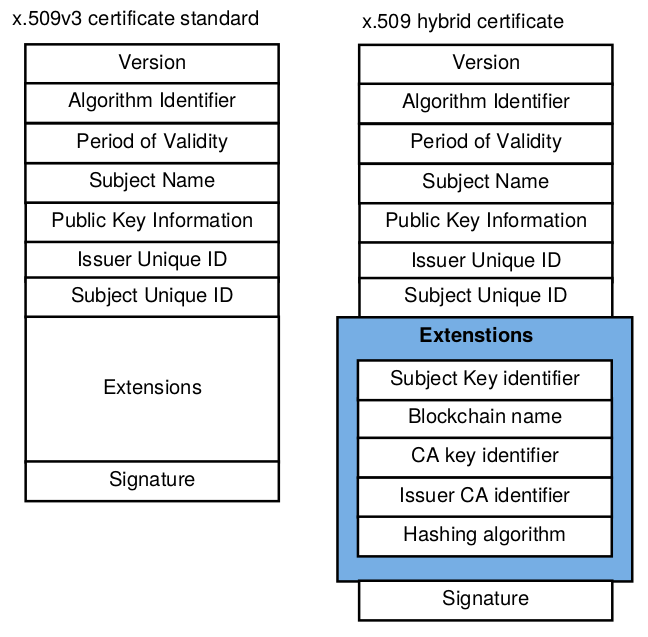
\includegraphics{figs/article_pki_blockchain.png}
%%\end{center}
%
%\end{frame}
%
%
%
%\begin{frame}{Data fields in Bitcoin-based blockchains}
%
%\begin{itemize}
%\item \mg{OP\_RETURN} field that can contain data
%\item Several blockchains could be used, such as Bitcoin or Namecoin
%%\vspace{2mm}
%\item Pros:
%\begin{itemize}
%\item Easy to implement, no hard fork required
%\end{itemize}
%\item Cons:
%\begin{itemize}
%\item No permissions: anyone can mine
%\item Bitcoin: small size of the field (80 bytes), only fingerprints of certificates
%\item Transaction fees
%\item No easy revocation protocol
%\item Burns bitcoins: they might not be used afterwards
%\item The whole blockchain has to be read each time
%\end{itemize}
%
%\end{itemize}
%
%\end{frame}
%

%
%\begin{frame}{New blockchain}
%\emph{here we describe the main points of our solution}
%
%\begin{itemize}
%\item Creation of a new blockchain with the \mg{Multichain} tool
%\item Pros:
%\begin{itemize}
%\item Very customizable
%\item Free transactions
%\item Data of any length
%\item Permission management
%\end{itemize}
%\item Cons:
%\begin{itemize}
%\item None :)
%\end{itemize}
%
%
%\end{itemize}
%\end{frame}


